%% Le lingue utilizzate, che verranno passate come opzioni al pacchetto babel. Come sempre, l'ultima indicata sarà quella primaria.
%% Se si utilizzano una o più lingue diverse da "italian" o "english", leggere le istruzioni in fondo.
\def\thudbabelopt{english,italian}
%% Valori ammessi per target: bach (tesi triennale), mst (tesi magistrale), phd (tesi di dottorato).
%% Valori ammessi per aauheader: '' (vuoto -> nessun header Alpen Adria Univeristat), aics (Department of Artificial Intelligence and Cybersecurity), informatics (Department of Informatics Systems). Il nome del dipartimento è allineato con la versione inglese del logo UniUD.
%% Valori ammessi per style: '' (vuoto -> stile moderno), old (stile tradizionale).
\documentclass[target=bach,aauheader=,style=]{thud}

%% --- Informazioni sulla tesi ---
%% Per tutti i tipi di tesi
% Scommentare quello di interesse, o mettete quello che vi pare
\course{Informatica}
%\course{Internet of Things, Big Data e Web}
%\course{Matematica}
%\course{Comunicazione Multimediale e Tecnologie dell'Informazione}
\title{Comparazione sperimentale \\ di algoritmi di cifratura lightweight \\ su microcontrollori embedded}
\author{Jacopo Plozner}
\supervisor{Prof.\ Marino Miculan}
%\cosupervisor{Arch.\ Rambaldo Melandri \and Dott.\ Giorgio Perozzi}
\tutor{Dott.\ Paolo Casoto}
%% Campi obbligatori: \title, \author e \course.
%% Altri campi disponibili: \reviewer, \tutor, \chair, \date (anno accademico, calcolato in automatico), \rights
%% Con \supervisor, \cosupervisor, \reviewer e \tutor si possono indicare più nomi separati da \and.
%% Per le sole tesi di dottorato:
%\phdnumber{313}
%\cycle{XXVIII}
%\contacts{Via della Sintassi Astratta, 0/1\\65536 Gigatera --- Italia\\+39 0123 456789\\\texttt{http://www.example.com}\\\texttt{inbox@example.com}}

%% --- Pacchetti consigliati ---
%% pdfx: per generare il PDF/A per l'archiviazione. Necessario solo per la versione finale
\usepackage[a-1b]{pdfx}
%% hyperref: Regola le impostazioni della creazione del PDF... più tante altre cose. Ricordarsi di usare l'opzione pdfa.
\usepackage[pdfa]{hyperref}
%% tocbibind: Inserisce nell'indice anche la lista delle figure, la bibliografia, ecc.

%% --- Stili di pagina disponibili (comando \pagestyle) ---
%% sfbig (predefinito): Apertura delle parti e dei capitoli col numero grande; titoli delle parti e dei capitoli e intestazioni di pagina in sans serif.
%% big: Come "sfbig", solo serif.
%% plain: Apertura delle parti e dei capitoli tradizionali di LaTeX; intestazioni di pagina come "big".
\usepackage{float} % figure EXACTLY here
\usepackage{MnSymbol} % simboli
\usepackage{algorithm} % algoritmi
\usepackage{algpseudocode} %pseudocodice

\usepackage{xcolor} % colori
\definecolor{mGreen}{rgb}{0,0.6,0}
\definecolor{mGray}{rgb}{0.5,0.5,0.5}
\definecolor{mPurple}{rgb}{0.58,0,0.82}
\definecolor{backgroundColour}{rgb}{0.95,0.95,0.92}

\usepackage{listings} % codice C
\lstdefinestyle{CStyle}{
	backgroundcolor=\color{backgroundColour},   
	commentstyle=\color{mGreen},
	keywordstyle=\color{magenta},
	numberstyle=\tiny\color{mGray},
	stringstyle=\color{mPurple},
	basicstyle=\footnotesize,
	breakatwhitespace=false,         
	breaklines=true,                 
	captionpos=b,                    
	keepspaces=true,                 
	numbers=left,                    
	numbersep=5pt,                  
	showspaces=false,                
	showstringspaces=false,
	showtabs=false,                  
	tabsize=2,
	language=C
}

\begin{document}
\maketitle

%% Dedica (opzionale)
\begin{dedication}
	Al mio cane,\par per avermi ascoltato mentre ripassavo le lezioni.
\end{dedication}

%% Ringraziamenti (opzionali)
\acknowledgements


%% Sommario (opzionale)
\abstract


%% Indice
\tableofcontents

%% Lista delle tabelle (se presenti)
%\listoftables

%% Lista delle figure (se presenti)
%\listoffigures

%% Corpo principale del documento
\mainmatter

%% Parte
%% La suddivisione in parti è opzionale; solitamente sono sufficienti i capitoli.
%\part{Parte}

%% Capitolo
\chapter{Introduzione}

    %% Sezione
    \section{Titolo della Sezione}


    %% Sottosezione
    \subsection{Sottosezione}

\chapter{Background}

    \section{Crittografia}
    La crittografia è la scienza, da alcuni definita anche \textit{arte}, che si occupa dello studio e della creazione di tecniche matematiche per la sicurezza di sistemi informatici e comunicazioni digitali.\cite{moderncrypto}\\
    Tra le molte tecniche troviamo i cifrari (cipher), algoritmi parametrizzati da una chiave (key) che trasformano un testo in chiaro (plaintext) in un testo cifrato (ciphertext).\\
    Le operazioni di cifratura \textit{E} (encryption) e decifratura \textit{D} (decryption) tramite la chiave \textit{K} e il rapporto tra plaintext \textit{P} e ciphertext \textit{C} possono essere rappresentati con le funzioni:
    \[E_K(P)=C \qquad , \qquad D_K(C)=P\]
    Un principio fondamentale della crittografia, che pone le basi per una progettazione sicura di un cifrario, è quello di Kerckhoffs:
    \begin{quote}
        La sicurezza di un sistema non deve dipendere dalla segretezza dell'algoritmo di cifratura usato, ma da quella della chiave.
    \end{quote}
    Claude Shannonn lo riformula con "Il nemico conosce il sistema" (\textit{Communication Theory of Secrecy Systems}); un cifrario quindi è considerato sicuro solo se garantisce la sua robustezza anche, e soprattutto, nel caso in cui un eventuale malintenzionato ne conosca tutti i dettagli implementativi.\\
    Questo consente ai crittografi di rendere pubbliche le loro scelte progettuali, in modo che il loro lavoro possa essere studiato e analizzato da altri esperti.
    
    Gli algoritmi di cifratura classici si dividono in due categorie: a chiave simmetrica e a chiave asimmetrica.

        \subsection{Crittografia simmetrica}
        Conosciuta anche come \textit{crittografia a chiave privata}, in questo scenario, due parti condividono una chiave segreta, che utilizzano per comunicare in modo cifrato.\\
        Le operazioni di cifratura e decifratura dei messaggi avvengono con la stessa chiave, da qui la definizione di \textit{simmetrica}. \\
        Una prima grande distinzione tra gli algoritmi in questa categoria si può fare sulla base di come operano sul messaggio: cifrari a blocco (\textit{Block ciphers}) e cifrari a flusso (\textit{Stream ciphers}).

            \subsubsection{Cifrari a blocco}
            Un cifrario a blocco è un algoritmo che opera su una quantità fissata di bit, detta appunto \textit{blocco}. \\
            Può essere descritto come una permutazione parametrizzata da una chiave\cite{moderncrypto}:
            \[F:\{0,1\}^b \times \{0,1\}^k \rightarrow \{0,1\}^b\]
            dove \textit{b} è la lunghezza del blocco e \textit{k} la lunghezza della chiave. 

            Diverse sono le architetture di cifrari a blocco presenti in letteratura, ma la maggior parte condivide le stesse idee base, teorizzate da Claude Shannon (\textit{A Mathematical Theory of Cryptography}, 1945):
            \begin{itemize}
                \item \textbf{Confusion}: il rapporto tra plaintext, ciphertext e chiave deve essere reso il piú complesso possibile. Questa proprietà viene raggiunta con l'utilizzo di tecniche di \textbf{sostituzione}, applicate all'intero messaggio diviso in gruppi di pochi bit, implementate tramite Look Up Table (S-Boxes)
                \item \textbf{Diffusion}: ogni cambiamento, anche il più piccolo, deve avere effetto su almeno metà blocco. Proprietá ottenuta tramite \textbf{permutazione} dei bit, grazie a semplici circuiti dedicati oppure una complicata implementazione software.
            \end{itemize}

            Architetture comuni:
            \begin{description}
                \item[Substitution-Permutation Networks (SPN)] Implementazione diretta del paradigma Confusion\&Diffusion\cite{moderncrypto}, sono infatti cifrari composti da divesi round di sostituzioni e permutazioni\cite{handcypto}.

                Prima dei round c'è la fase detta \textbf{Key Schedule}, in cui la chiave principale (\textit{master key}) viene usata per generare le sotto-chiavi utilizzate in ciascun round (\textit{round keys}).\\
                Ogni round è composto solitamente dalle seguenti fasi\cite{moderncrypto}:                
                \begin{enumerate}
                    \item Round key mixing: la round key corrispondente viene sommata al messaggio. \[M = M \oplus RK_i\]
                    \item Substitution: sostituzione dei byte del messaggio $(M:m_0||\ ...\ ||m_n)$ sulla base delle S-Box. \[M=S(m_0)||\ ...\ ||S(m_n)\]
                    \item Permutation: permutazione dei bit di M.
                \end{enumerate}
                L'output di ciascun round è l'input del successivo.\\
                Dopo l'ultimo round il messaggio è sommato all'ultima sotto-chiave.
                \begin{figure}[htbp]
                    \centering
                    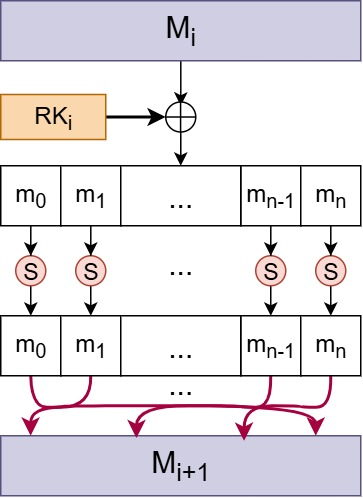
\includegraphics[width=0.5\linewidth]{img/spn_round.jpg}
                    \caption{SPN round}
                    \label{fig:placeholder}
                \end{figure}
                \item[Feistel Networks \cite{moderncrypto}] Approccio teorizzato da Horst Feistel (\textit{Cryptography and Computer Privacy}, 1973), al contrario degli SPN, presenta il vantaggio di poter utilizzare come componente base una funzione non invertibile \textit{RF} (\textit{round function}).\\
                Anche in questo caso, operando a round, è presente una fase inziale di \textit{key schedule} per espandere la \textit{master key K} nelle relative \textit{round keys $RK_i$}.\\
                Questi cifrari operano iterativamente sul messaggio, considerandolo come due parti di lunghezza uguale ($M_i:L_i||R_i$), nel seguente modo:
                \begin{enumerate}
                    \item $L_{i+1} = R_i$
                    \item $R_{i+1} = L_i \oplus RF_{RK_i}(R_i)$
                \end{enumerate}
                \begin{figure}[htbp]
                    \centering
                    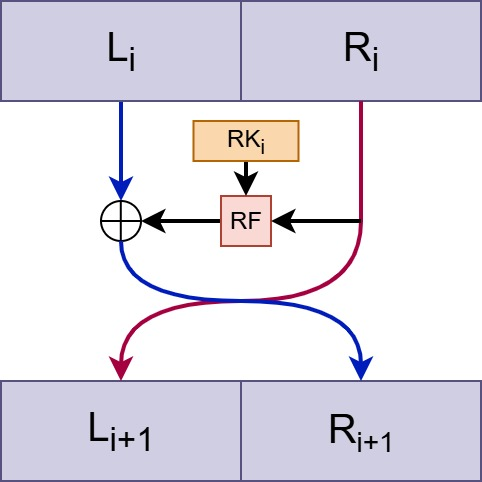
\includegraphics[width=0.5\linewidth]{img/feistel_round.jpg}
                    \caption{Feistel Network round}
                    \label{fig:placeholder}
                \end{figure}
                \item[Add-Rotate-XOR (ARX)\cite{sparx}] Classe di cifrari progettati utilizando soltanto semplici operazioni di \textit{addizione modulare} ($\boxplus$), \textit{rotazione} ($\lll, \ggg$) e \textit{XOR} ($\oplus$).
            \end{description}
            
            Di per sé non è una soluzione sicura, soprattutto in presenza di più blocchi da cifrare, in quanto presenta un comportamento deterministico: applica, a parità di chiave, sempre la stessa permutazione. Occorre adottare delle particolari tecniche, chiamate \textit{Modes of Operation}, che utilizzano il cifrario a blocco come primitiva e non come unica risorsa. \cite{handcypto, computernet}
            % modes
            
            \subsubsection{Cifrari a flusso}
            Un cifrario a flusso è un algoritmo che cifra un messaggio combinandolo con un flusso pseudocasuale di simboli (\textit{keystream}). Ogni simbolo del plaintext è cifrato con il simbolo corrispondente del keystream.\\
            La componente base di un cifrario a flusso è solitamente un \textit{LFSR} (\textit{linear-feedback shift register}), uno strumento utilizzato per la generazione pseudocasuale di numeri, con buone proprietà statistiche. Un LFSR consiste in un array di registri da un bit ciascuno, i cui valori ne rappresentano lo stato. Lo stato è aggiornato ad ogni intervallo dato, shiftando i valori dei registri verso destra, mentre il nuovo valore del primo registro da sinistra è calcolato tramite lo XOR di un sottoinsieme dei valori attuali. In un dato momento, il valore dell'ultimo registro a destra rappresenta l'output del LFSR.\cite{moderncrypto}
            \begin{figure}[htbp]
                \centering
                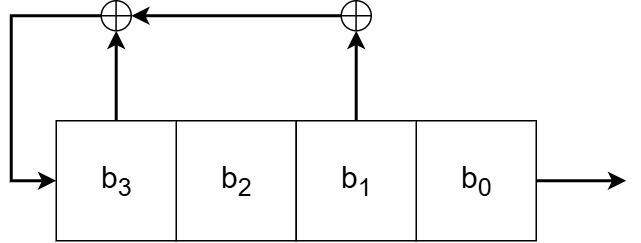
\includegraphics[width=0.5\linewidth]{img/lfsr.jpg}
                \caption{LFSR}
                \label{fig:placeholder}
            \end{figure}
        \subsection{Crittografia asimmetrica}

    \section{Sistemi embedded}
    Un sistema embedded può essere definito come "un sistema informatico progettato e costruito esclusivamente per il suo scopo"\cite{embeddedsys}.
    I sistemi embedded spaziano tra i più disparati oggetti: dall'uso quotidiano (elettrodomestici), ai veicoli, ai sensori intelligenti (come nel caso di questa tesi), fino a scopi militari (missili).\\
    I computer \textit{integrati} in questi sistemi sono detti \textit{microcontrollori}\cite{architetture}.
    
    	\subsection{Vincoli}
    	%costi, hardware, software
    	Essendo progettati per un compito specifico, i sistemi embedded offrono meno supporto e presentano spesso numerosi vincoli. La necessità di produzione su larga scala e il fatto di rientrare nel budget del dispositivo in cui sono integrati richiedono ai progettisti un'attenta analisi dei \textit{costi}. La riduzione dei costi si riflette direttamente sui vincoli \textit{hardware} dei dispositivi, soprattutto in termini di RAM, ROM, velocità del processore, periferiche e consumo energetico. Come spesso accade, l'ottimizzazione di queste risorse risulta un problema complesso, richiedendo dei compromessi: codice più veloce richiede più spazio, aumentando la velocità della CPU aumentano di conseguenza i consumi, rimuovendo le periferiche non strettamente necessarie si guadagna in spazio e consumi, e molti altri.
    	Dal lato software, invece, possono essere richieste garanzie di \textit{real-time}, determinismo, oppure di tolleranza ai guasti.\cite{embeddedsys}
    	\subsection{Programmazione}
    	La sviluppo di codice embedded richiede diverse competenze, tra cui: conoscenza approfondita dell'hardware presente nel dispositivo, padronanza della programmazione a basso livello, soprattutto nella gestione della memoria, abilità nel bilanciare le richieste applicative con i vincoli del sistema.
    	Al contrario di quello che accade nei dispositivi general-purpose, inoltre, una errata gestione software può causare danni alle componenti hardware, anche gravi.
    		\subsubsection{Linguaggi}
    		Avendo risorse limitate, i sistemi embedded non sono dotati di compilatore, il codice che eseguono è \textit{cross-compilato} su un altro dispositivo e successivamente trasferito nella memoria integrata. I produttori di microprocessori solitamente forniscono ambienti di sviluppo dedicati con cross-compiler proprietari, ma sono presenti anche alternative GNU.
    		Le tool-chain embedded, nella maggior parte dei casi, supportano solo linguaggi come C o C++, con funzionalità e librerie limitate (es. supporto ridotto per aritmetica floating-point).
			\subsubsection{Debug}
			Altra questione delicata è quella del debugging, che, similmente alla compilazione, richiede un \textit{cross-debugger}. Questi particolari programmi sono eseguiti su un dispositivo esterno e comunicano con il microprocessore target tramite interfacce e periferiche dedicate (es. JTAG).
			Le funzionalità di debug devono essere esplicitamente supportate dal processore, attraverso hardware specifico, come per esempio registri riservati ai breakpoint (hardware breakpoint).
			
			\begin{figure}[h]
				\centering
				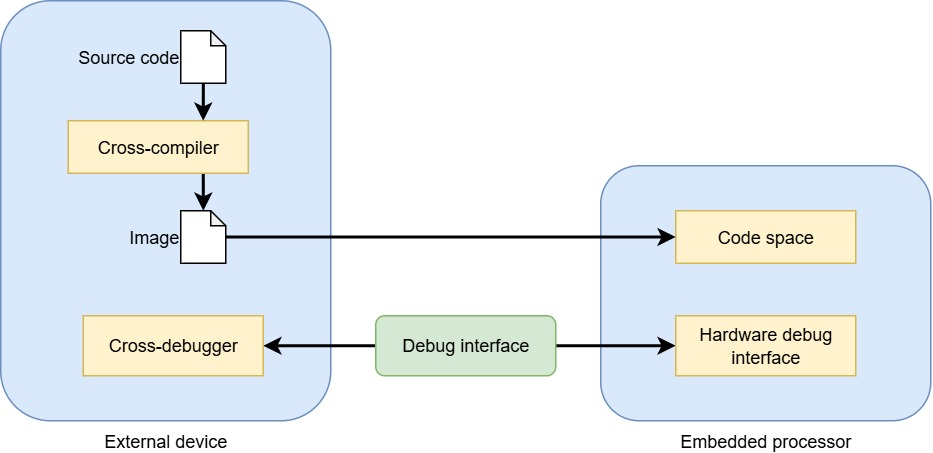
\includegraphics[width=0.5\linewidth]{img/cross-compiler-debugger.jpg}
				\caption{Comunicazione con microprocessore embedded}
				\label{fig:placeholder}
			\end{figure}
			    		
\chapter{Algoritmi}
	\section{Cifrari a blocco}
		\subsection{AES\cite{aes}}
		L'Advanced Encryption Standard specifica un algoritmo crittografico approvato dal FIPS (Federal Information Processing Standards), scelto al termine di una competizione indetta dal NIST (US National Institute of Standards and Technology), che vide come vincitore il cifrario presentato da Vincent Rijmen e Joan Daemen: Rijndael. Sia durante il processo di selezione che dopo essere stato adottato come standard, questo algoritmo ha ricevuto un intenso studio da parte dei crittoanalisti. Anche per questo motivo, AES risulta una scelta eccellente per sistemi che richiedano segretezza: libero, standardizzato, efficiente e altamente sicuro. \cite{moderncrypto}
			\subsubsection{Design}
			Le operazioni dell'algoritmo sono effettuate su un array bi-dimensionale ($4 \times 4$), definito state. Il cuore dell'algoritmo è caratterizzato da una serie di round, durante cui, in sequenza, vengono applicate queste trasformazioni:
			\begin{itemize}
				\item \Call{SubBytes}{\null} : trasformazione invertibile e non-lineare, descritta da una S-box e ottenuta tramite la sostituzione indipendente dei byte dello state.
				\begin{lstlisting}[style=CStyle]
static void sub_bytes(uint8_t *state) {
	for(uint16_t i = 0; i < 16; i++) {	
		state[i] = sbox[state[i]];
	}
}\end{lstlisting}
				\item \Call{ShiftRows}{\null} : shift dei byte che compongono le ultime tre righe dello state.
				\begin{lstlisting}[style=CStyle]
static void shift_rows(uint8_t *state) {
	uint8_t tmp;
	
	// row 1
	tmp = state[13];
	state[13] = state[1];
	state[1] = state[5];
	state[5] = state[9];
	state[9] = tmp;
	
	// row 2
	tmp = state[14];
	state[14] = state[6];
	state[6] = tmp;
	tmp = state[10];
	state[10] = state[2];
	state[2] = tmp;
	
	// row 3
	tmp = state[3];
	state[3] = state[15];
	state[15] = state[11];
	state[11] = state[7];
	state[7] = tmp;
}\end{lstlisting}
				\item \Call{MixColumns}{\null} : moltiplicazione in $GF(2^8)$ tra lo state e una matrice fissata.

				\begin{lstlisting}[style=CStyle]
static void mix_columns(uint8_t *state) {
	uint8_t new_s0;
	uint8_t new_s1;
	uint8_t new_s2;
	uint8_t new_s3;
	for(uint16_t c = 0; c < 4; c++) {
		new_s0 = xtimes(state[4*c]) ^ (xtimes(state[4*c+1]) ^ 
				state[4*c+1]) ^ state[4*c+2] ^ state[4*c+3];
		new_s1 = state[4*c] ^ xtimes(state[4*c+1]) ^ 
				(xtimes(state[4*c+2]) ^ state[4*c+2]) ^ state[4*c+3];
		new_s2 = state[4*c] ^ state[4*c+1] ^ 
				xtimes(state[4*c+2]) ^ (xtimes(state[4*c+3]) ^ state[4*c+3]);
		new_s3 = (xtimes(state[4*c]) ^ state[4*c]) ^ 
				state[4*c+1] ^ state[4*c+2] ^ xtimes(state[4*c+3]);
		
		state[4*c] = new_s0;
		state[4*c+1] = new_s1;
		state[4*c+2] = new_s2;
		state[4*c+3] = new_s3;
	}
}\end{lstlisting}
				\item \Call{AddRoundKey}{\null} : somma (bitwise XOR) tra ciascuna colonna e la relativa word della round key corrispondente.

				\begin{lstlisting}[style=CStyle]
static void add_round_key(uint8_t *state, uint8_t *rk) {
	for(uint16_t k = 0; k < 16; k++) {
		state[k] ^= rk[k];
	}
}\end{lstlisting}
			\end{itemize}
			
			\begin{algorithm}
				\caption{Pseudocodice AES}
				\begin{algorithmic}
					\Procedure{Cipher}{$in, Nr, w$}
						\State {$state \gets in$}
						\State {$state \gets \Call{AddRoundKey}{state,w[0 \cdots 3]}$}
						\For{$round=1$ \textbf{to} $Nr-1$}
							\State {$state \gets \Call{SubBytes}{state}$}
							\State {$state \gets \Call{ShiftRows}{state}$}
							\State {$state \gets \Call{MixColumns}{state}$}
							\State {$state \gets \Call{AddRoundKey}{state,w[4*round \cdots 4*round+3]}$}
						\EndFor
						\State {$state \gets \Call{SubBytes}{state}$}
						\State {$state \gets \Call{ShiftRows}{state}$}
						\State {$state \gets \Call{AddRoundKey}{state,w[4*Nr \cdots 4*Nr+3]}$}
						\Return state
					\EndProcedure
				\end{algorithmic}
			\end{algorithm}
			
			\begin{algorithm}
				\caption{Codice C AES-128}
				\begin{lstlisting}[style=CStyle]
void AES128_encrypt(uint8_t *plaintext, uint8_t *round_key, uint8_t *ciphertext) {
	for(uint16_t b = 0; b < 16; b++) {
		ciphertext[b] = plaintext[b];
	}
	
	add_round_key(ciphertext, round_key);
	round_key += 16;
	
	for(uint16_t r = 1; r < 10; r++) {
		sub_bytes(ciphertext);
		shift_rows(ciphertext);
		mix_columns(ciphertext);
		add_round_key(ciphertext, round_key);
		round_key += 16;
	}
	
	sub_bytes(ciphertext);
	shift_rows(ciphertext);
	add_round_key(ciphertext, round_key);
}\end{lstlisting}
			\end{algorithm}
			
			Le round key sono generate tramite la procedura \Call{KeyExpansion}{\null}, in modo ricorsivo, a partire dalla chiave principale.\\
			In questa fase, due sono le trasformazioni applicate:
			\[\Call{RotWord}{[a_0,a_1,a_2,a_3]} = [a_1,a_2,a_3,a_0],\]
			\[\Call{SubWord}{[a_0,a_1,a_2,a_3]} = [S(a_0),S(a_1), S(a_2), S(a_3)].\]
			\begin{algorithm}
				\caption{Pseudocodice Key Expansion}
				\begin{algorithmic}
					\Procedure{KeyExpansion}{key}
						\State {$i \gets 0$}
						\While{$i \le Nk-1 $}
							\State {$w[i] \gets key[i]$}
							\State {$i \gets i+1$}
						\EndWhile
						\While{$i \le 4*Nr + 3$}
							\State {$temp \gets w[i-1]$}
							\If{$i \mod Nk = 0$}
								\State {$temp \gets \Call{SubWord}{}(\Call{RotWord}{temp}) \oplus Rcon[i/Nk]$}
							\ElsIf{$(Nk \gtr 6) \wedge (i \mod Nk = 4)$}
								\State {$temp \gets \Call{SubWord}{temp}$}
							\EndIf
							\State {$w[i] \gets w[i - Nk] \oplus temp$}
							\State {$i \gets i+1$}
						\EndWhile
						\State {\textbf{return} $w$}
					\EndProcedure
				\end{algorithmic}
			\end{algorithm}
			\begin{algorithm}
				\caption{Codice C Key Expansion AES-128}
\begin{lstlisting}[style=CStyle]
void AES128_compute_round_keys(uint8_t *key, uint8_t *round_key) {
	for(uint16_t k = 0; k < 16; k++) {
		round_key[k] = key[k];
	}
	
	uint8_t tmp[4];
	for(uint16_t i = 4; i < 44; i++) {
		tmp[0] = round_key[4*(i-1)];
		tmp[1] = round_key[4*(i-1) + 1];
		tmp[2] = round_key[4*(i-1) + 2];
		tmp[3] = round_key[4*(i-1) + 3];
		
		if(!(i & 0x3)) { // i % Nk (4) == 0
			rot_word(tmp);
			sub_word(tmp);
			tmp[0] ^= rcon[i >> 2]; // i/Nk (4)
		}
		
		round_key[4*i] = round_key[4*(i-4)] ^ tmp[0];
		round_key[4*i + 1] = round_key[4*(i-4) + 1] ^ tmp[1];
		round_key[4*i + 2] = round_key[4*(i-4) + 2] ^ tmp[2];
		round_key[4*i + 3] = round_key[4*(i-4) + 3] ^ tmp[3];
	}
}\end{lstlisting}
			\end{algorithm}
			\subsubsection{Crittoanalisi}
			\begin{center}
				\begin{tabular}{ |c|c|c| } 
					\hline
					Attacco & Complessità & Fonte \\ 
					\hline
					\hline
					Biclique (AES-128) & $2^{126.1}$ & \cite{aes_biclique} \\ 
					\hline
					Related-key (AES-256) & $2^{99.5}$ & \cite{aes_relatedkey} \\ 
					\hline
					Side channel & pratica & \cite{aesside, aesfault}\\
					\hline
				\end{tabular}
			\end{center}
		\subsection{CLEFIA\cite{clefia}}
		CLEFIA è un cifrario proprietario sviluppato da Sony, sfruttando le ultime scoperte in ambito di crittoanalisi.
			\subsubsection{Design}
			La struttura base è data da una particolare estensione di rete Feistel (Type-2 generalized Fesitel network): a 4-rami e con due funzioni ($F_0, F_1$) per round. Queste funzioni adottano \textit{Diffusion Switching Mechanism}\cite{clefiadsm}: utilizzano due diverse matrici di diffusione per aumentare l'immunità ad attacchi differenziali e lineari.\\
			La struttura della particolare rete Feistel adottata è descritta come:\\
			\begin{algorithm}[htbp]
				\caption{Generaized Fesitel Network}
				\begin{algorithmic}
					\Procedure{$GFN_{4,r}$}{$RK, X$}
						\State {$T_0|T_1|T_2|T_3 \gets X_0|X_1|X_2|X_3$}
						\For{$i=0$ \textbf{to} $r-1$}
							\State {$T_1 \gets T_1 \oplus F_0(RK_{2i},T_0)$}
							\State {$T_3 \gets T_3 \oplus F_1(RK_{2i+1},T_2)$}
							\State {$T_0|T_1|T_2|T_3 \gets T_1|T_2|T_3|T_0$}
						\EndFor
						\State {\textbf{return} $T_3|T_0|T_1|T_2$}
					\EndProcedure
				\end{algorithmic}
			\end{algorithm}
			
			\begin{minipage}[c]{0.45\textwidth}
				\noindent
				\centering
				\begin{algorithm}[H]
					\caption{$F_0$}
					\begin{algorithmic}
						\Procedure{$F_0$}{$RK,x$}
						\State {$T \gets RK \oplus x$}
						\State {$T \gets S_0(T_0)|S_1(T_1)|S_0(T_2)|S_1(T_3)$}
						\State {\textbf{return} $M_0 \times ^tT$}
						\EndProcedure
					\end{algorithmic}
				\end{algorithm}
			\end{minipage}
			\begin{minipage}[c]{0.45\textwidth}
				\noindent
				\centering
				\begin{algorithm}[H]
					\caption{$F_1$}
					\begin{algorithmic}
						\Procedure{$F_1$}{$RK,x$}
						\State {$T \gets RK \oplus x$}
						\State {$T \gets S_1(T_0)|S_0(T_1)|S_1(T_2)|S_0(T_3)$}
						\State {\textbf{return} $M_1 \times ^tT$}
						\EndProcedure
					\end{algorithmic}
				\end{algorithm}
			\end{minipage}\\		
			Sono inoltre presenti due S-box, basate su strutture algebriche differenti, scelta che \textit{prevede} di aumentare la resistenza ad attacchi algebrici.\\
			
			\begin{algorithm}
				\caption{pseudocodice CLEFIA}
				\begin{algorithmic}
					\Procedure{Clefia$_r$}{$WK,RK,P$}
					\State {$T_0|T_1|T_2|T_3 \gets P_0|(P_1 \oplus WK_0)|P_2|(P_3 \oplus WK_1)$}
					\State {$T_0|T_1|T_2|T_3 \gets GFN_{4,r}(RK,T)$}
					\State {\textbf{return} $T_0|(T_1 \oplus WK_2)|T_2|(T_3 \oplus WK_3)$}
					\EndProcedure
				\end{algorithmic}
			\end{algorithm}

			La key schedule é divisa in due fasi:
			\begin{enumerate}
				\item generazione di una chiave intermedia \textit{L}
				\item espansione di \textit{L} per generare whitening key $WK$ e round key $RK_i$
			\end{enumerate}
			
			\begin{algorithm}
				\caption{pseudocodice Key Expansion CLEFIA-128}
				\begin{algorithmic}
					\Procedure{KeyExpansion}{K}
						\State {$L \gets GFN_{4,12}(CON_{0..23}, K)$}
						\State {$WK \gets K$}
						\For{$i = 0$ \textbf{to} $8$}
							\State {$T \gets L \oplus (CON_{24+4i}|CON_{24+4i+1}|CON_{24+4i+2}|CON_{24+4i+3})$}
							\State {$L \gets L[7..63] | L[121..127] | L[0..6] | L[64..120]$}
							\If{$i$ is odd}
								\State {$T \gets T \oplus K$}
							\EndIf
							\State {$RK_{4i} \gets T$}
						\EndFor
					\EndProcedure
				\end{algorithmic}
			\end{algorithm}
			
			\subsubsection{Crittoanalisi}
			Diversi studi consentono di affermare che Clefia è resistente alle moderne tecniche di crittoanalisi.\cite{clefiaanal}
			\begin{center}
				\begin{tabular}{ |c|c|c| } 
					\hline
					Attacco & Complessità & Fonte \\ 
					\hline 
					\hline
					Reduced-round (15) improbable differential & $2^{126.83}$ & \cite{clefiadiff} \\
					\hline
					Side channel & pratica & \cite{clefiafault}\\
					\hline
				\end{tabular}
			\end{center}
		\subsection{LEA\cite{lea}}
		Lightweight Encryption Algorithm (LEA) è un cifrario sviluppato dalla Corea del Sud, da cui è inoltre adottato come standard nazionale. Obiettivo principale è quello di risultare efficiente sia in implementazioni software che in quelle hardware.
			\subsubsection{Design}
			LEA consiste di sole operazioni ARX su word di 32 bit. La word-size è stata scelta dai progettisti sulla base della convinzione che in futuro le operazioni a 32 bit saranno implementate efficientemente anche su dispositivi con risorse limitate.
			La cifratura è divisa in tre fasi: inizializzazione, round iterativi e finalizzazione.
			\begin{algorithm}
				\caption{pseudocodice LEA}
				\begin{algorithmic}
					\Procedure{LEA}{P,RK}
						\State {$X_0 \gets P$}
						\For{$i=0$ \textbf{to} $r-1$}
							\State {$X_{i+1}[0] \gets LROT_9((X_i[0] \oplus RK_i[0]) \boxplus (X_i[1] \oplus RK_i[1]))$}
							\State {$X_{i+1}[1] \gets RROT_5((X_i[1] \oplus RK_i[2]) \boxplus (X_i[2] \oplus RK_i[3]))$}
							\State {$X_{i+1}[2] \gets RROT_3((X_i[2] \oplus RK_i[4]) \boxplus (X_i[3] \oplus RK_i[5]))$}
							\State {$X_{i+1}[3] \gets X_i[0]$}
						\EndFor
						\State {$C \gets X_r$}
						\State {\textbf{return} $C$}
					\EndProcedure
				\end{algorithmic}
			\end{algorithm}
			
			\begin{algorithm}
				\caption{Codice C LEA-128}
\begin{lstlisting}[style=CStyle]
void LEA_encrypt(uint32_t *plaintext, uint32_t *round_key, uint32_t *ciphertext) {
	uint32_t x[4] = {plaintext[0], plaintext[1], plaintext[2], plaintext[3]};
	
	for(uint16_t i = 0; i < 24; i++) {
		uint32_t tmp = x[0];
		uint16_t rk_i = 6 * i;
		x[0] = LROT((x[0] ^ round_key[rk_i]) + (x[1] ^ round_key[rk_i + 1]), 9);
		x[1] = RROT((x[1] ^ round_key[rk_i + 2]) + (x[2] ^ round_key[rk_i + 3]), 5);
		x[2] = RROT((x[2] ^ round_key[rk_i + 4]) + (x[3] ^ round_key[rk_i + 5]), 3);
		x[3] = tmp;
	}
	
	ciphertext[0] = x[0];
	ciphertext[1] = x[1];
	ciphertext[2] = x[2];
	ciphertext[3] = x[3];
}\end{lstlisting}
			\end{algorithm}
			La struttura della key schedule è semplice, senza mix tra word diverse o avalanche effect, ma non per questo poco sicura. Come per la cifratura, le operazioni sono ARX, con l'aggiunta dell'utilizzo di costanti $\delta$.
			La semplicità è ancora una volta ricercata per consentire implementazioni efficienti.
			\begin{algorithm}
				\caption{pseudocodice key schedule LEA-128}
				\begin{algorithmic}
					\Procedure{KeySchedule}{K}
						\State {$T \gets K$}
						\For{$i = 0$ \textbf{to} 23}
							\State {$T[0] \gets LROT_1(T[0] \boxplus LROT_i(\delta[i \mod 4]))$}
							\State {$T[1] \gets LROT_3(T[1] \boxplus LROT_{i+1}(\delta[i \mod 4]))$}
							\State {$T[2] \gets LROT_6(T[2] \boxplus LROT_{i+2}(\delta[i \mod 4]))$}
							\State {$T[3] \gets LROT_{11}(T[3] \boxplus LROT_{i+3}(\delta[i \mod 4]))$}
							\State {$RK_i \gets T[0]|T[1]|T[2]|T[1]|T[3]|T[1]$}
						\EndFor
					\EndProcedure
				\end{algorithmic}
			\end{algorithm}
			\begin{algorithm}
				\caption{Codice C key schedule LEA-128}
\begin{lstlisting}[style=CStyle]
void LEA_compute_round_keys(uint32_t *key, uint32_t *round_key) {
	uint32_t t[4] = {key[0], key[1], key[2], key[3]};
	
	for(uint16_t i = 0; i < 24; i++) {
		t[0] = LROT(t[0] + LROT(constants[i & 3], i), 1);
		t[1] = LROT(t[1] + LROT(constants[i & 3], i + 1), 3);
		t[2] = LROT(t[2] + LROT(constants[i & 3], i + 2), 6);
		t[3] = LROT(t[3] + LROT(constants[i & 3], i + 3), 11);
		
		uint16_t rk_i = 6 * i;
		round_key[rk_i] = t[0];
		round_key[rk_i + 1] = t[1];
		round_key[rk_i + 2] = t[2];
		round_key[rk_i + 3] = t[1];
		round_key[rk_i + 4] = t[3];
		round_key[rk_i + 5] = t[1];
	}
}\end{lstlisting}
			\end{algorithm}
			
			\subsubsection{Crittoanalisi}
			Lo sviluppo di LEA è stato guidato anche dall'obiettivo di resistere a tutti gli attacchi esistenti e garantire un certo margine di sicurezza futura. Sia $R$ il numero minimo di round per resistere a tutte le tecniche di crittoanalisi, LEA ne prevede $3R/2$ in previsione di nuove tipologie di attacchi che potrebbero emergere in futuro.\\
			Al momento non esistono attacchi full-round noti.
			\begin{center}
				\begin{tabular}{ |c|c|c| } 
					\hline
					Attacco & Complessità & Fonte \\ 
					\hline 
					\hline
					Reduced-round (13) differential & $2^{127}$ & \cite{leadiff} \\
					\hline
					Reduced-round (15) boomerang & $2^{116.3}$ & \cite{lea} \\
					\hline
					Reduced-round (14) differential-linear & - & \cite{lea} \\
					\hline
				\end{tabular}
			\end{center}
		\subsection{PRINCE\cite{prince}}
			PRINCE è un cifrario ottimizzato rispetto alla latenza su  hardware; consente infatti implementazioni full-unrolled, con cifratura in un solo ciclo di clock.
			\subsubsection{Design}
			L'obiettivo dei progettisti di PRINCE era creare un cifrario sulla base dei seguenti criteri: cifratura istantanea, bassa latenza, costi hardware moderati, decifratura ottenibile con minor overhead possibile.
			Per ottenere i primi due, sono necessari round in numero ridotto e con logica non troppo complessa: un critical-path leggero consente infatti di impiegare una velocità di clock maggiore.
			Gli ultimi due criteri, invece, sono consentite grazie alla particolare proprietà di $\alpha$-reflection: la decifratura corrisponde ad un cifratura con una chiave ricavata da quella principale.\\
			PRINCE è un cifrario a blocchi di 64 bit, con una chiave da 128 bit $k = k_0 || k_1$. La chiave è estesa a 192 bit:
			\[(k_0||k'_0||k_1) := (k_0 || (k_0 \ggg 1) \oplus (k_0 \gg 63) || k_1)\]\\
			La struttura base è detta \textit{FX-construction}: le sotto chiavi $k_0$ e $k'_0$ sono usate come whitening key, mentre $k_1$ è usata nei 12 round del costrutto chiamato PRINCE$_{core}$.
			\begin{figure}[htbp]
				\centering
				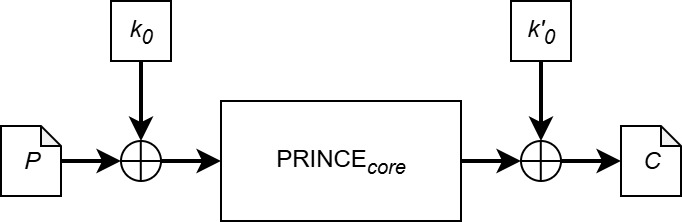
\includegraphics[width=0.5\linewidth]{img/princefx.jpg}
				\caption{PRINCE FX-construct}
				\label{fig:placeholder}
			\end{figure}
			Ogni round prevede le seguenti trasformazioni dello stato:
			\begin{enumerate}
				\item \textbf{$k_1$-add}: somma (XOR) con la sotto-chiave.
				\item \textbf{S-Layer}: sostituzione con S-box $S$ a 4 bit.
\begin{lstlisting}[style=CStyle]
	static uint64_t state_sbox(uint64_t state, uint16_t inverse) {
		uint64_t result = 0;
		for(uint16_t i = 0; i < 16; i++) {	
			uint8_t nibble = (state >> (i * 4)) & 0xf;
			result |= ((uint64_t) sbox[inverse][nibble]) << (i * 4);
		}
		
		return result;
}\end{lstlisting}
				\item \textbf{(M/M')-Layer}: moltiplicazione con matrice $M$ o $M'$. Essendo usata nel round centrale, $M'$ deve essere un'involuzione; $M$ si ottiene invece con la combinazione tra $M'$ e una permutazione $SR$: $M = SR \circ M' $.
				\[SR:(0,1,2,3,4,5,6,7,8,9,10,11,12,13,14,15) \rightarrow (0,5,10,15,4,9,14,3,8,13,2,7,12,1,6,11) \]
				Le seguenti matrici sono utilizzate per costruire $M'$:
				\[M_0 = 
				\begin{pmatrix}
					0000\\
					0100\\
					0010\\
					0001
				\end{pmatrix},
				M_1 =
				\begin{pmatrix}
					1000\\
					0000\\
					0010\\
					0001
				\end{pmatrix},
				M_2 =
				\begin{pmatrix}
					1000\\
					0100\\
					0000\\
					0001
				\end{pmatrix},
				M_3 =
				\begin{pmatrix}
					1000\\
					0100\\
					0010\\
					0000
				\end{pmatrix}
				\]
				Da cui:
				\[ \hat{M^{(0)}} = 
				\begin{pmatrix}
					M_0\ M_1\ M_2\ M_3\\
					M_1\ M_2\ M_3\ M_0\\
					M_2\ M_3\ M_0\ M_1\\
					M_3\ M_0\ M_1\ M_2
				\end{pmatrix},
				\hat{M^{(1)}} = 
				\begin{pmatrix}
					M_1\ M_2\ M_3\ M_0\\
					M_2\ M_3\ M_0\ M_1\\
					M_3\ M_0\ M_1\ M_2\\
					M_0\ M_1\ M_2\ M_3
				\end{pmatrix}
				\]
				Infine, $M'$ è ottenuta costruendo una matrice $64 \times 64$ con $(\hat{M^{(0)}} , \hat{M^{(1)}}, \hat{M^{(1)}}, \hat{M^{(0)}})$ come blocchi diagonali.
\begin{lstlisting}[style=CStyle]
static uint64_t linear_transform(uint64_t state) {
	uint64_t col0 = 0;
	uint64_t col1 = 0;
	uint64_t col2 = 0;
	uint64_t col3 = 0;
	
	for(uint16_t bit = 63; bit > 47; bit--) {
		if((state >> bit) & 0x1) {
			col0 ^= mhat[0][15 - (bit & 0xf)];
		}
	}
	for(uint16_t bit = 47; bit > 31; bit--) {
		if((state >> bit) & 0x1) {
			col1 ^= mhat[1][15 - (bit & 0xf)];
		}
	}
	for(uint16_t bit = 31; bit > 15; bit--) {
		if((state >> bit) & 0x1) {
			col2 ^= mhat[1][15 - (bit & 0xf)];
		}
	}
	for(int16_t bit = 15; bit > -1; bit--) {
		if((state >> bit) & 0x1) {
			col3 ^= mhat[0][15 - (bit & 0xf)];
		}
	}
	
	return (col0 << 48) | (col1 << 32) | (col2 << 16) | col3;
}

static uint64_t shift_rows(uint64_t state ,uint16_t inverse) {
	uint64_t new_state = 0;
	for(uint16_t i = 0; i < 16; i++) {	
		uint8_t nibble = (state >> ((15 - sr[inverse][i]) * 4)) & 0xf;
		new_state |= ((uint64_t) nibble) << (60 - i*4);
	}
	
	return new_state;
}\end{lstlisting}
				\item \textbf{$RC_i$-add}: somma (XOR) con la relativa costante. Le costanti sono scelte in modo che per $0 \le i \le 11$, $RC_i \oplus RC_{11-i} = \alpha = 0xc0ac29b7c97c50dd$; $RC_0 = 0$ e $RC_{1...5}$ sono derivate dalla parte decimale di $\pi$.
			\end{enumerate}
				\begin{figure}[htbp]
				\centering
				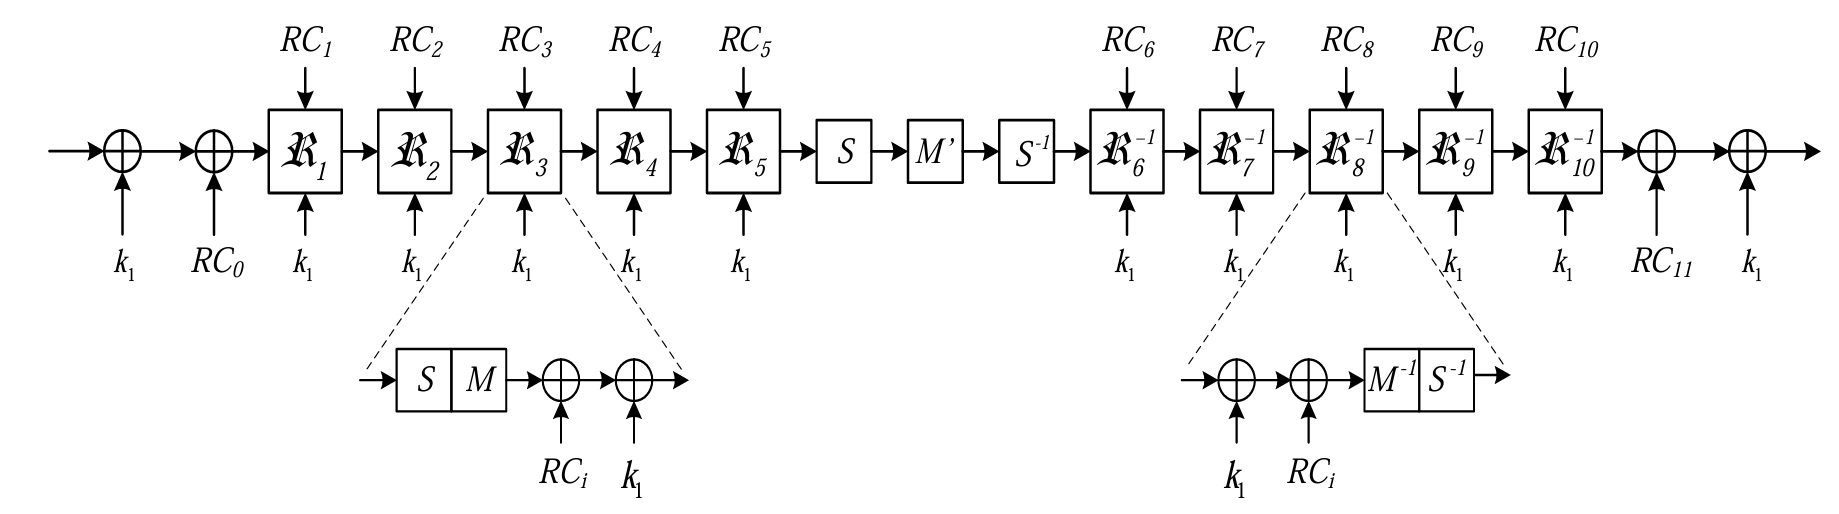
\includegraphics[width=0.5\linewidth]{img/princestruct.jpg}
				\caption{PRINCE rounds}
				\label{fig:placeholder}
			\end{figure}
			Dal fatto che $M'$ sia un'involuzione e che $0 \le i \le 11$, $RC_i \oplus RC_{11-i} = \alpha$ si deduce che:
			\[D_{(k_0||k'_0||k_1)}(\cdot) = E_{(k'_0||k_0||k_1 \oplus \alpha)}(\cdot) \tag{\text{$\alpha$-reflection}}\]
			
						\begin{algorithm}
				\caption{Codice C PRINCE}
\begin{lstlisting}[style=CStyle]
void PRINCE_encrypt(uint64_t *plaintext, uint64_t *key, uint64_t *ciphertext) {
	uint64_t k[3] = {
		key[0],
		key[1],
		((key[0] >> 1) | (key[0] << 63)) ^ (key[0] >> 63)
	};
	
	prince_block(plaintext, k, ciphertext);
}

void PRINCE_decrypt(uint64_t *ciphertext, uint64_t *key, uint64_t *plaintext) {
	uint64_t k[3] = {
		((key[0] >> 1) | (key[0] << 63)) ^ (key[0] >> 63),
		key[1] ^ 0xc0ac29b7c97c50dd, // alpha
		key[0]
	};
	
	prince_block(ciphertext, k, plaintext);
}

void prince_block(uint64_t *m, uint64_t *k, uint64_t *c) {
	uint64_t state = *m;
	state ^= k[0];
	
	//-----------------
	//	PRINCE core
	//
	state ^= k[1] ^ rc[0];
	
	// Forward
	for(uint16_t r = 1; r < 6; r++) {
		state = state_sbox(state, 0);
		
		state = linear_transform(state);
		state = shift_rows(state, 0);
		
		state ^= rc[r] ^ k[1];
	}
	
	// Central
	state = state_sbox(state, 0);
	state = linear_transform(state);
	state = state_sbox(state, 1);
	
	// Backward
	for(uint16_t r = 6; r < 11; r++) {
		state ^= k[1] ^ rc[r];
		
		state = shift_rows(state, 1);
		state = linear_transform(state);
		
		state = state_sbox(state, 1);
	}
	
	state ^= rc[11] ^ k[1];
	//
	//-----------------
	
	state ^= k[2];
	
	*c = state;
}\end{lstlisting}
			\end{algorithm}
			\subsubsection{Crittoanalisi}
			Nel 2016 è stata indetta una competizione per incoraggiare l'analisi di PRINCE (\textit{Prince challenge}), che ha portato alla scoperta di diversi attacchi reduced-round. Sono emersi in seguito altri attacchi full-round.
			\begin{center}
				\begin{tabular}{ |c|c|c| } 
					\hline
					Attacco & Complessità & Fonte \\ 
					\hline 
					\hline
					Linear & $2^{125.67}$ & \cite{princesec}\\
					\hline
					Related-key & $2^{64}$ & \cite{princesec}\\
					\hline
				\end{tabular}
			\end{center}
		\subsection{QARMAv2\cite{qarmav2}}
			\subsubsection{Design}
			\subsubsection{Crittoanalisi}
		\subsection{Sparx\cite{sparx}}
			\subsubsection{Design}
			\subsubsection{Crittoanalisi}
		\subsection{Speck\cite{speck}}
			\subsubsection{Design}
			\subsubsection{Crittoanalisi}
		\subsection{XTEA}
			\subsubsection{Design}
			\subsubsection{Crittoanalisi}
	\section{Cifrari a flusso}
		\subsection{Ascon\cite{ascon}}
			\subsubsection{Design}
			\subsubsection{Crittoanalisi}
		\subsection{ChaCha20\cite{chacha20}}
			\subsubsection{Design}
			\subsubsection{Crittoanalisi}
		\subsection{Hummingbird-2\cite{hummingbird2}}
			\subsubsection{Design}
			\subsubsection{Crittoanalisi}
		\subsection{Lesca\cite{lesca}}
			\subsubsection{Design}
			\subsubsection{Crittoanalisi}
\chapter{Test e valutazione}

\chapter{Conclusione}



%% Fine dei capitoli normali, inizio dei capitoli-appendice (opzionali)
\appendix

%\part{Appendici}

\chapter{Appendice}


%% Parte conclusiva del documento; tipicamente per riassunto, bibliografia e/o indice analitico.
\backmatter

%% Riassunto (opzionale)
%\summary

%% Bibliografia (praticamente obbligatoria)
\bibliographystyle{plain_\languagename}%% Carica l'omonimo file .bst, dove \languagename è la lingua attiva.
%% Nel caso in cui si usi un file .bib (consigliato)
\bibliography{thud}

%% Nel caso di bibliografia manuale, usare l'environment thebibliography.

%% Per l'indice analitico, usare il pacchetto makeidx (o analogo).

\end{document}